\newpage
\section{Aufbau und Durchführung}\label{sec:aufbau-und-durchfuehrung}

Im Experiment wird ein Dia mit einem Helium-Neon-Laser\footnote{$\lambda = \SI{635}{\nano\m}$} bestrahlt, auf das ein weißer Spalt belichtet wurde, welcher den Laser beugt. Das Beugungsmuster wird in \SI{93}{\cm} Entfernung mithilfe einer Photodiode vermessen, die auf einem Reiter sitzt. Der Reiter lässt sich in \SI{10}{\mu\m}-Schritten verschieben. Die Diode ist an ein analoges Strommessgerät angeschlossen.

Auf dem Dia befinden sich drei verschieden breite Spalte und ein Doppelspalt, die alle nach obigen Verfahren vermessen wurden. Zusätzlich wurden mit einem digitalem Mikroskop die Spaltabstände nachgemessen\footnote{Behelfsmäßig wurde ein fester Rahmen auf dem Bildschirm als ``Skala'' benutzt, der mit der beim Mikroskop mitgelieferten Eichkarte verglichen wurde. Die verschieden großen Zoomstuden wurden per Schlussrechung umgerechnet.}.

%\begin{figure}
%  \centering
%  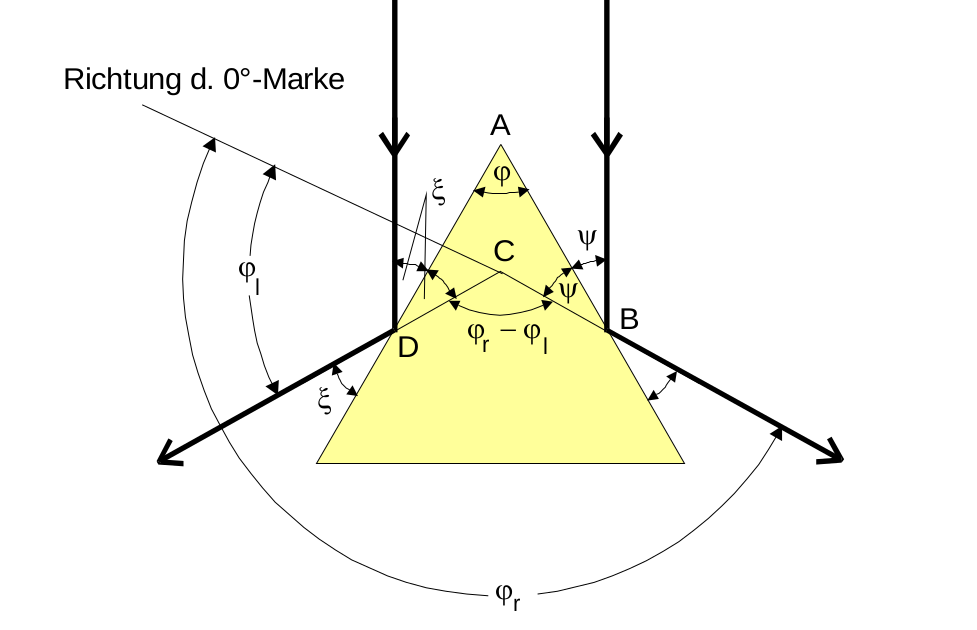
\includegraphics[width=0.4\textheight]{../figures/phi.png}
%  \caption{Schematische Darstellung zur Messung des Winkels~$\varphi$ an der brechenden Kante eines Prismas. [Skript V402]}
%\label{fig:prism}
%\end{figure}
